%!TEX root = ../thesis.tex

\section{Descentralizacion}  %Title of the First Chapter

La descentralización se ha utilizado en  estrategia, gestión y gobierno durante mucho tiempo. La idea básica consiste en distribuir el control y la autoridad a las periferias en lugar de que una autoridad central tenga el control total de la organización. Esto resulta en varios beneficios para las organizaciones, como una mayor eficiencia, una toma de decisiones más rápida, y una menor carga para la gerencia de bajo y alto nivel~\cite{bashir2017mastering}.

A pesar de no ser un concepto nuevo, la descentralización empieza a tomar gran importancia en el mundo tecnológico, al ser el servicio principal y central brindado por plataformas \textit{blockchain}. Si bien los sistemas descentralizados  y distribuidos tienen mucho en común su principal diferencia radica en que, en los sistemas distribuidos todavía existe una autoridad central que gobierna todo el sistema, mientras que en un sistema descentralizado, no existe tal autoridad. Se podría decir que el \textit{blockchain} es la manera perfecta de proveer una  plataforma que no necesite ningún intermediario o entidad de control, y puede funcionar mediante la interacción de varios participantes o nodos, los cuales definen o validan el estado actual del sistema mediante mecanismos de consenso, específicamente mecanismos de consenso descentralizados que son una verdadera innovación en el paradigma descentralizado. La Figura~\ref{blockchain_descentralziation} compara los tres tipos de redes.

\begin{figure}[h]
    \centering
    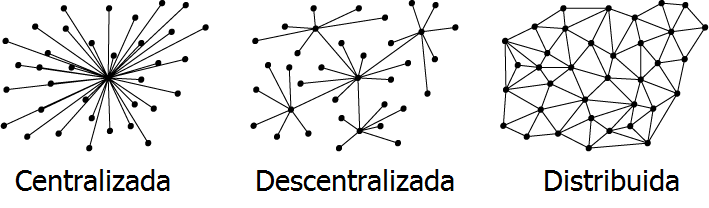
\includegraphics[width=0.8\textwidth]{descentralizacion.png}
     \caption{Diferencia entre redes centralizadas, descentralizadas y distribuidas}
    \label{blockchain_descentralziation}
\end{figure}

Existen dos métodos de descentralización conocidos que pueden ser utilizados:
\begin{itemize}
    \item Desintermediación: El término es bastante común y de uso frecuente en economía e implica la eliminación de intermediarios en una cadena de suministro, o la eliminación de los intermediarios en relación con una transacción o una serie de transacciones~\cite{lin2015infinite}. Un ejemplo de este término aplicado al \textit{blockchain} es la famosa plataforma Bitcoin, en donde se puede  enviar dinero (token) a un conocido, amigo o familiar con solo saber su dirección, eliminando la  necesidad de que una o varias entidades bancarias validen y realicen la transferencia hasta la cuenta destino.
    \item Por competencia:  En este método, un grupo de proveedores de servicios compiten entre sí para ser seleccionados por el sistema para la prestación de servicios. Este paradigma no logra la descentralización completa, pero en cierta medida asegura que un intermediario o proveedor de servicios no esté monopolizando el mismo. En el contexto de tecnología \textit{blockchain}, se puede prever un sistema en el cual los contratos inteligentes pueden elegir un proveedor de datos o nodo candidato externo de una gran lista de proveedores en función de su reputación, puntaje previo, revisiones y calidad del servicio. Esto no dará lugar a una descentralización completa, pero permite que los contratos inteligentes hagan una elección libre en base a los criterios mencionados anteriormente. De esta forma, se crea un entorno de competencia entre los proveedores de servicios, en el que compiten entre sí para convertirse en el proveedor de datos de elección~\cite{bashir2017mastering}.
\end{itemize}

Existe un marco de trabajo que se puede  utilizar para evaluar los requisitos de descentralización de una variedad de elementos en el contexto de la tecnología \textit{blockchain} y que fue propuesto por Arvind Narayanan entre otros~\cite{narayanan2012critical}. El marco básicamente propone cuatro preguntas que se deben responder para generar una idea clara de cómo se puede descentralizar un sistema:
\begin{enumerate}
    \item ¿Qué está siendo descentralizado?
Hace referencia al sistema que se está descentralizando o se quiere descentralizar.
    \item ¿Qué nivel de descentralización se requiere?
Se responde especificando el nivel de descentralización requerido, el cual puede ser aplicando a alguno de los dos métodos discutidos anteriormente: Desintermediacion (descentralizacion total) o Por Competencia (descentralización parcial).
    \item ¿Qué \textit{blockchain} se usa?
Selección de plataforma \textit{blockchain}  adecuada para una aplicación en particular.
    \item ¿Qué mecanismo de seguridad se usa?
Finalmente, es necesario responder a una pregunta clave sobre el mecanismo de seguridad,  en otras palabras cómo se puede garantizar la seguridad de un sistema descentralizado. Un buen ejemplo de esto puede ser la Atomicidad, por el cual la transacción se ejecuta por completo o no se ejecuta en absoluto. El objetivo es asegurar la integridad del sistema.
\end{enumerate}

\subsection{Tipos de organismos descentralizados}
\begin{itemize}
    \item Las organizaciones descentralizadas (DOs, por sus siglas en inglés de {\it Descentralized Organizations})  son programas de software que se ejecutan en una \textit{blockchain} y requiere la interacción constante entre personas o integrantes de la organización para efectuar funciones y operaciones relacionadas a la lógica de negocios. Una vez que una DO, en la forma de un contrato inteligente o un conjunto de contratos inteligentes, se agrega al \textit{blockchain}, el mismo se descentraliza y las partes interactúan entre sí en función del código definido en el software de DO.
    \item Las organización autónoma descentralizada (DAO, por sus siglas en inglés {\it Decentralized Autonomous Organizations})  es básicamente lo mismo que una DO con la diferencia principal que las DAO son autónomos, lo que significa que son completamente automáticos y contienen una lógica artificialmente inteligente, mientras que los DO carecen de esta característica y dependen de los datos humanos para ejecutar la lógica comercial.
    \item Las corporaciones autónomas descentralizadas (DAC, por sus siglas en inglés {\it Decentralized Autonomous	Corporations}) son un concepto similar, pero se consideran un subconjunto de las  DAO. Las definiciones de DAC y DAO se pueden superponer en varios escenarios, sin embargo usualmente difieren en  que los DAO en general se consideran sin fines de lucro, mientras que los DAC pueden ganar dinero a través de acciones ofrecidas a los participantes y mediante el pago de dividendos. Estas corporaciones pueden ejecutar un negocio automáticamente sin intervención humana en función de la lógica programada dentro de ellos.
    \item Las sociedades autónomas descentralizadas (DAS, por sus siglas en inglés {\it Decentralized Autonomous	Societies}) son un concepto mediante el cual sociedades enteras pueden funcionar en un \textit{blockchain} con la ayuda de múltiples contratos inteligentes complejos y una combinación de DAO y aplicaciones descentralizadas (DAPP, por sus siglas en inglés {\it Decentralized	Application}) que funcionan de forma autónoma. Este modelo no significa un enfoque fuera de la ley, ni se basa en una ideología totalmente libertaria; en cambio, muchos servicios que ofrece un gobierno se pueden entregar a través del \textit{blockchain}, como sistemas de tarjetas de identidad del gobierno, emisión de pasaportes y registros de escrituras, matrimonios y nacimientos.
    \item Las aplicaciones descentralizadas (DAPP) son programas de software que pueden ejecutarse en su propia \textit{blockchain}, utilizar otra \textit{blockchain}  o utilizar sólo protocolos de una solución de \textit{blockchain} existente. Todas los DAO, DAC y DO son básicamente aplicaciones descentralizadas que se ejecutan en la parte superior de un \textit{blockchain} en una red punto a punto. Este es el último avance en tecnología con respecto a la descentralización.

\end{itemize}